%%%%%%%%%%%%%%%%%%%%%%%%%%%%%%%%%%%%%%%%%
% Programming/Coding Assignment
% LaTeX Template
%
% This template has been downloaded from:
% http://www.latextemplates.com
%
% Original author:
% Ted Pavlic (http://www.tedpavlic.com)
%
% Note:
% The \lipsum[#] commands throughout this template generate dummy text
% to fill the template out. These commands should all be removed when 
% writing assignment content.
%
% This template uses a Perl script as an example snippet of code, most other
% languages are also usable. Configure them in the "CODE INCLUSION 
% CONFIGURATION" section.
%
%%%%%%%%%%%%%%%%%%%%%%%%%%%%%%%%%%%%%%%%%

%----------------------------------------------------------------------------------------
%	PACKAGES AND OTHER DOCUMENT CONFIGURATIONS
%----------------------------------------------------------------------------------------

\documentclass{article}

\usepackage{fancyhdr} % Required for custom headers
\usepackage{lastpage} % Required to determine the last page for the footer
\usepackage{extramarks} % Required for headers and footers
\usepackage[usenames,dvipsnames]{color} % Required for custom colors
\usepackage{graphicx} % Required to insert images
\usepackage{subcaption}
\usepackage{listings} % Required for insertion of code
\usepackage{courier} % Required for the courier font
\usepackage{lipsum} % Used for inserting dummy 'Lorem ipsum' text into the template

% Margins
\topmargin=-0.45in
\evensidemargin=0in
\oddsidemargin=0in
\textwidth=6.5in
\textheight=9.0in
\headsep=0.25in

\linespread{1.1} % Line spacing

% Set up the header and footer
\pagestyle{fancy}
\lhead{\hmwkAuthorName} % Top left header
\chead{\hmwkClass\ (\hmwkClassTime): \hmwkTitle} % Top center head
%\rhead{\firstxmark} % Top right header
\lfoot{\lastxmark} % Bottom left footer
\cfoot{} % Bottom center footer
\rfoot{Page\ \thepage\ of\ \protect\pageref{LastPage}} % Bottom right footer
\renewcommand\headrulewidth{0.4pt} % Size of the header rule
\renewcommand\footrulewidth{0.4pt} % Size of the footer rule

\setlength\parindent{0pt} % Removes all indentation from paragraphs

%----------------------------------------------------------------------------------------
%	CODE INCLUSION CONFIGURATION
%----------------------------------------------------------------------------------------

\definecolor{MyDarkGreen}{rgb}{0.0,0.4,0.0} % This is the color used for comments
\lstloadlanguages{Perl} % Load Perl syntax for listings, for a list of other languages supported see: ftp://ftp.tex.ac.uk/tex-archive/macros/latex/contrib/listings/listings.pdf
\lstset{language=Perl, % Use Perl in this example
        frame=single, % Single frame around code
        basicstyle=\small\ttfamily, % Use small true type font
        keywordstyle=[1]\color{Blue}\bf, % Perl functions bold and blue
        keywordstyle=[2]\color{Purple}, % Perl function arguments purple
        keywordstyle=[3]\color{Blue}\underbar, % Custom functions underlined and blue
        identifierstyle=, % Nothing special about identifiers                                         
        commentstyle=\usefont{T1}{pcr}{m}{sl}\color{MyDarkGreen}\small, % Comments small dark green courier font
        stringstyle=\color{Purple}, % Strings are purple
        showstringspaces=false, % Don't put marks in string spaces
        tabsize=5, % 5 spaces per tab
        %
        % Put standard Perl functions not included in the default language here
        morekeywords={rand},
        %
        % Put Perl function parameters here
        morekeywords=[2]{on, off, interp},
        %
        % Put user defined functions here
        morekeywords=[3]{test},
       	%
        morecomment=[l][\color{Blue}]{...}, % Line continuation (...) like blue comment
        numbers=left, % Line numbers on left
        firstnumber=1, % Line numbers start with line 1
        numberstyle=\tiny\color{Blue}, % Line numbers are blue and small
        stepnumber=5 % Line numbers go in steps of 5
}

% Creates a new command to include a perl script, the first parameter is the filename of the script (without .pl), the second parameter is the caption
\newcommand{\perlscript}[2]{
\begin{itemize}
\item[]\lstinputlisting[caption=#2,label=#1]{#1.pl}
\end{itemize}
}

%----------------------------------------------------------------------------------------
%	DOCUMENT STRUCTURE COMMANDS
%	Skip this unless you know what you're doing
%----------------------------------------------------------------------------------------

% Header and footer for when a page split occurs within a Part environment
\newcommand{\enterPartHeader}[1]{
%\nobreak\extramarks{#1}{#1 continued on next page\ldots}\nobreak
%\nobreak\extramarks{#1 (continued)}{#1 continued on next page\ldots}\nobreak
}

% Header and footer for when a page split occurs between Part environments
\newcommand{\exitPartHeader}[1]{
%\nobreak\extramarks{#1 (continued)}{#1 continued on next page\ldots}\nobreak
%\nobreak\extramarks{#1}{}\nobreak
}

\setcounter{secnumdepth}{0} % Removes default section numbers
\newcounter{ProjectPartCounter} % Creates a counter to keep track of the number of Parts
\setcounter{ProjectPartCounter}{0}

\newcommand{\ProjectPartName}{}
\newenvironment{ProjectPart}[1][Part \arabic{ProjectPartCounter}]{ % Makes a new environment called ProjectPart which takes 1 argument (custom name) but the default is "Part #"
\stepcounter{ProjectPartCounter} % Increase counter for number of Parts
\renewcommand{\ProjectPartName}{#1} % Assign \ProjectPartName the name of the Part
\section{\ProjectPartName} % Make a section in the document with the custom Part count
\enterPartHeader{\ProjectPartName} % Header and footer within the environment
}{
\exitPartHeader{\ProjectPartName} % Header and footer after the environment
}

\newcommand{\PartAnswer}[1]{ % Defines the Part answer command with the content as the only argument
\noindent\framebox[\columnwidth][c]{\begin{minipage}{0.98\columnwidth}#1\end{minipage}} % Makes the box around the Part answer and puts the content inside
}

\newcommand{\ProjectSectionName}{}
\newenvironment{ProjectSection}[1]{ % New environment for sections within Project Parts, takes 1 argument - the name of the section
\renewcommand{\ProjectSectionName}{#1} % Assign \ProjectSectionName to the name of the section from the environment argument
\subsection{\ProjectSectionName} % Make a subsection with the custom name of the subsection
\enterPartHeader{\ProjectPartName\ [\ProjectSectionName]} % Header and footer within the environment
}{
\enterPartHeader{\ProjectPartName} % Header and footer after the environment
}

%----------------------------------------------------------------------------------------
%	NAME AND CLASS SECTION
%----------------------------------------------------------------------------------------

\newcommand{\hmwkTitle}{Assignment1} % Assignment title
\newcommand{\hmwkDueDate}{Friday,\ February\ 3,\ 2016} % Due date
\newcommand{\hmwkClass}{CSC411} % Course/class
\newcommand{\hmwkClassTime}{L0101} % Class/lecture time
\newcommand{\hmwkAuthorName}{Xiaodi Lu} % Your name

%----------------------------------------------------------------------------------------
%	TITLE PAGE
%----------------------------------------------------------------------------------------

\title{
\vspace{2in}
\textmd{\textbf{\hmwkClass:\ \hmwkTitle}}\\
\normalsize\vspace{0.1in}\small{Due\ on\ \hmwkDueDate}\\
\vspace{0.1in}
\vspace{3in}
}

\author{\textbf{\hmwkAuthorName}}
%\date{} % Insert date here if you want it to appear below your name

%----------------------------------------------------------------------------------------

\begin{document}

\maketitle
\clearpage
%----------------------------------------------------------------------------------------
%	PART 1
%----------------------------------------------------------------------------------------

% To have just one Part per page, simply put a \clearpage after each Part

\begin{ProjectPart}

\noindent \textit{Dataset description}

The data-set consists of $1918$ various size of colored uncropped images of a few actors and actresses, and grayscale images of the same data set but resized and cropped out the faces to $32\times 32$-pixel. The cropped images of actors and actresses are random and the faces of theirs can be a side face, or there are some hair covering it, or the face is not completely in the image and there is considerable variation in the appearance of the faces. However, examining the dataset, it appears that there are more nicely cropped faces than other images, and most of the face are facing the front.  Most faces do not align with each other, and the faces can have various emotions on the faces and facing all sort of directions. A random sample of $3$ ``cropped out faces"s is shown in Figure 1, 2, and 3. 


\begin{figure}[h]   
    \minipage{0.32\textwidth}
    
\includegraphics[width=\linewidth]{baldwin22}
    \caption{This face is not cropped properly leaving part of the face out of the picture}
    \endminipage
    \hspace{10px}
    \minipage{0.32\textwidth}
    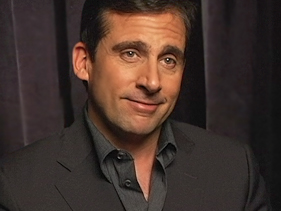
\includegraphics[width=\linewidth]{carell62}
    \caption{This face is cropped perfectly, no unnecessary background in the picture}
    \endminipage
    \hspace{10px}
    \minipage{0.32\textwidth}
    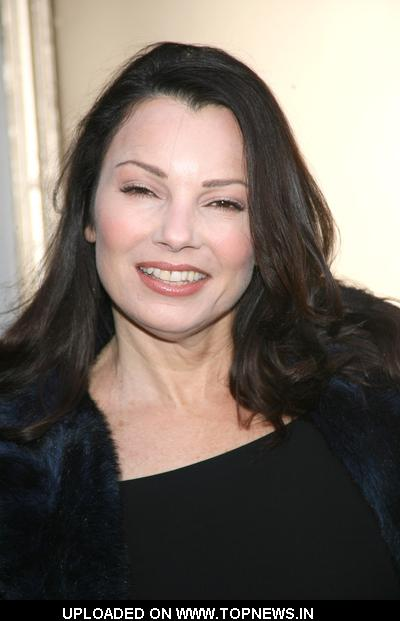
\includegraphics[width=\linewidth]{drescher140}
    \caption{This face is also cropped perfectly and the person is smiling in the picture, unlike the others.}
    \endminipage
\end{figure}

\pagebreak
The uncropped dataset images might be taken when people are not looking in the camera, or smilling at the camera, or can be taken for a cover photo of a magazine, which there could be letters and other stuff covering some part of the face. And the faces usually do not align with each other.  A random sample of $3$ ``cropped out faces"s is shown in Figure 4, 5, and 6. 
\begin{figure}[h]   
    \minipage{0.32\textwidth}
    
\includegraphics[width=\linewidth]{butler18}
    \caption{This face is not cropped properly leaving part of the face out of the picture}
    \endminipage
    \hspace{10px}
    \minipage{0.32\textwidth}
    
\includegraphics[width=\linewidth]{ferrera20}
    \caption{This face is cropped perfectly, no unnecessary background in the picture}
    \endminipage
    \hspace{10px}
    \minipage{0.32\textwidth}
    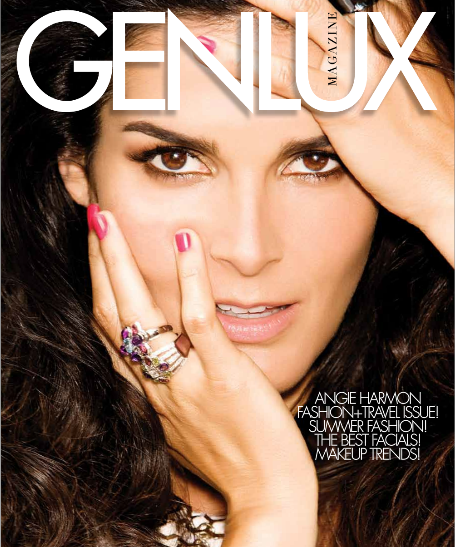
\includegraphics[width=\linewidth]{harmon35}
    \caption{This face is also cropped perfectly and the person is smiling in the picture, unlike the others.}
    \endminipage
\end{figure}





\end{ProjectPart}
\clearpage
%----------------------------------------------------------------------------------------
%	Part 2
%----------------------------------------------------------------------------------------

\begin{ProjectPart}
\noindent \textit{Separate the dataset into three non-overlapping parts}\\

First, I created a folder for each actor, then I take all images from the cropped folder and separate them by  actors using the image's file name and put it in the actor's list in the dictionary, and random each list.  Then I loop over each actor's image list in the dictionary to copy the first 100 images of each list into the actor's training set subfolder, the next 10 images into the test set subfolder, and the next 10 images to the validation set subfolder, and the folders are all created in the actor's folder.






\end{ProjectPart}
\clearpage
%----------------------------------------------------------------------------------------
%	Part 3
%----------------------------------------------------------------------------------------

\begin{ProjectPart}
\noindent \textit{Build a classifier to distinguish pictures of Bill Hader form pictures of Steve Carell}

The cost function I used is the following function $f$
\begin{lstlisting}
def f(x, y, theta):
    return 0.0025*sum( (y - np.dot(x, theta)) ** 2)
\end{lstlisting}
which is this function put into code 
$\frac{1}{2m}\sum_{i}(\theta^{T}x^{(i)} - y^{(i)})^{2}$\\

On the training set:\\
Value of the cost function: 0.047\\
Percentage of images that were correctly classified: 0.910\\
On the validation set:\\
Value of the cost function: 0.003\\
Percentage of images that were correctly classified: 0.900\\
\nopagebreak
\newline We used the function $grad\_descent$ to compute the classifier and the function $class_or_correct$ to construct the data.

\begin{lstlisting}
def df(x, y, theta):
    return -0.005 * np.dot(x.T, (y - np.dot(x, theta)))
    
def grad_descent(f, df, x, y, init_t, alpha):
    t = init_t.copy()
    max_iter = 30000
    iter  = 0
    while iter < max_iter:
        t -= alpha*df(x, y, t)
        iter += 1
    return 
    
def class_or_correct(size, set, flag): 
    '''flag = 1 :classifiy
       flag = 0 :correction
    '''
    x = np.empty(shape=[0, 1024])
    y = np.array([[1 for v in range(size/2)]])
    y1 = np.array([[0 for p in range(size/2)]])
    y = np.concatenate((y, y1), 1)
    y = np.reshape(y, (size,1))
    one = np.array([[1 for q in range(size)]])
    one = np.reshape(one, (size,1))
    
    hader = os.listdir("hader/" + set)
    carell = os.listdir("carell/" + set)
    
    for i in range(size):
        if (i < size/2):
            im = imread("hader/" + set + hader[i])[:,:,0]
        else :
            im = imread("carell/"+ set + carell[i-size/2])[:,:,0]
        im = np.reshape(im, (1, 1024))
        x = np.concatenate((x, im), 0)

    x = np.concatenate((one, x), 1)
    if flag:
        t = np.zeros([1025, 1])  
        return grad_descent(f, df, x, y, t, 5*1e-10)
    else:
        correction = 0
        expect = np.dot(x, new_t)
        
        for i in range(size):
            if i < size/2:
                if expect[i] >= 0.5:
                    correction += 1
            else: 
                if expect[i] < 0.5:
                    correction += 1
        print"cost: %.3f\n" %(f(x, y, new_t))
        print"Percentage: %.3f\n" % (correction/float(size))
        
def part3(size):
    global new_t
    new_t = class_or_correct(size, "trainning_set/", 1)
    class_or_correct(size, "trainning_set/", 0)
    class_or_correct(10, "validation_set/", 0)
\end{lstlisting}

I made sure that the image pixel array for Hader would be labeled as $1$ and Carell would be labeled as $0$.  And the two actors are in their half of the matrix in $x$.  And the alpha shouldn't be too large. When I set the alpha too large, the $t$ in the $grad\_descent$ function would jump further and further away from the minimum point that we want.  When that happens I kept on trying to descrease alpha and stop at the point where the cost is considerably small.  The iteration being too large could result in overfitting, so I kept the $max\_iteration$ not too large and not too small either, otherwise the performance would be bad.\\


\end{ProjectPart}
\clearpage

%----------------------------------------------------------------------------------------
%	Part 4
%----------------------------------------------------------------------------------------

\begin{ProjectPart}
\noindent \textit{Display the $\theta$s that you obtain by training using the full training dataset, and by training using a training set that contains only two images of each actor}


Hypothesis Function: $h_\theta (x) = \theta_0 + \theta_1 x_1 + ... + \theta_n x_n$
\begin{figure}[h]   
    \minipage{0.49\textwidth}
    
\includegraphics[width=\linewidth]{full}
    \caption{The theta image using full training dataset}
    \endminipage
    \hspace{10px}
    \minipage{0.49\textwidth}
    
\includegraphics[width=\linewidth]{small}
    \caption{The theta image using a training subset of two images each actor}
    \endminipage
\end{figure}



\end{ProjectPart}
\clearpage



%----------------------------------------------------------------------------------------
%	Part 5
%----------------------------------------------------------------------------------------

\begin{ProjectPart}
\noindent \textit{Demonstrate Overfitting}


\begin{lstlisting}
act =['Fran Drescher', 'America Ferrera', 'Kristin Chenoweth', 'Alec Baldwin', 
                                                        'Bill Hader', 'Steve Carell']
                                                        
act_test = ['Gerard Butler', 'Daniel Radcliffe', 'Michael Vartan', 'Lorraine Bracco', 
                                                        'Peri Gilpin', 'Angie Harmon']
\end{lstlisting}

\includegraphics[width=\linewidth]{Performance_Plot}
Note: the $x-axis$'s label is wrong it should be the training example size.
The blue line is the performance percentage of the classifier on the training set of the actors in $act$.  The yellow line is the performance percentage of the classifier on the validation set of the actors in $act$. The green line is the performance percentage of the classifier on the test set of the actors in $act\_test$.  With the classifier built by each iteration.\\

The performance of the $act\_test$ is increasing as iteration increase except at the last point where it went down which is a result of overfitting.
\end{ProjectPart}
\clearpage



%----------------------------------------------------------------------------------------
%	Part 6
%----------------------------------------------------------------------------------------

\begin{ProjectPart}
\noindent \textit{A different way of classifying inputs}



        \includegraphics[width=0.98\linewidth]{6a}


        \includegraphics[width=0.98\linewidth]{6b}\\
        $X$ is $n\times m$ dimension\\
        $\theta$ is $n\times k$ dimension\\
        $Y$ is $k\times m$ dimension\\
        $\theta^{T}$ is $k\times n$ dimension\\
        $n$ is the number of pixels\\
        $m$ is the number of training examples\\
        $k$ is the number of possible labels\\

\newpage
6.c\\
The cost function from Part 6 and the vectorized gradient function in Python.\\
\begin{lstlisting}
def cost(x, y, theta):
    #x = vstack( (ones((1, x.shape[1])), x))
    return sum( (np.dot(theta.T,x) - y) ** 2)
 
def derive(x, y, theta):
    #x = vstack( (ones((1, x.shape[1])), x))
    return 2 * np.dot(x, (np.dot(theta.T, x) - y).T)
    
def vectorized_grad_descent(f, df, x, y, init_t, alpha):
    t = init_t.copy()
    max_iter = 30000
    iter  = 0
    while iter < max_iter:
        t -= alpha*df(x, y, t)
        # if iter % 500 == 0:
        #     print "Iter", iter
        #     print "x = (%.2f, %.2f, %.2f), f(x) = %.2f" % (t[0], t[1], t[2], f(x, y, t)) 
        #     print "Gradient: ", df(x, y, t), "\n"
        iter += 1
    return t
\end{lstlisting}

6.d\\
The cost function from Part 6 and the vectorized gradient function in Python.\\
\begin{lstlisting}
def part6(p, q):
    h = 5*1e-11
    x = np.ones([1025, 600])
    y = np.ones([6, 600])
    theta = np.ones([1025, 6])
    theta_h = np.ones([1025, 6])
    theta_h[p, q] += h 
    print (cost(x, y, theta_h) - cost(x, y, theta))/h
    print derive(x, y, theta)[p, q]
\end{lstlisting}
I printed out the derivative calculated using the finite difference and the dervie function on several function call $(p, q) = (3,5)$ finite difference output is  $1230239.86816$ derive function output is $1228800.0$
$(p, q) = (6,1)$ finite difference output is  $1230239.86816$ derive function output is $1228800.0$
$(p, q) = (16,4)$ finite difference output is  $1230239.86816$ derive function output is $1228800.0$
\end{ProjectPart}
\clearpage




%----------------------------------------------------------------------------------------
%	Part 7
%----------------------------------------------------------------------------------------

\begin{ProjectPart}
\noindent \textit{Perform face recognition}\\

Alpha is $5*1e-11$. I first tried setting alpha to $5*1e-10$, but the $t$ in the function kept jumping further and further away from the minimum point. On second try, I used a smaller alpha $5*1e-11$, and it worked out fine.\\

The $max\_iteration$ was not changed from part 5, since the performance percentage were high enough on both set, which implies overfitting did not occur.\\

$X$ is our dataset the first entry on every column is the bias and the rest is its pixel array we got from the image.  Every column is a training example therefore the dimension is $1025\times600$.\\

$Y$ is the expected output from the function using our classifier, in other words, we are hoping the theta we get can help us recognize every person, therefore it is $[1, 0, 0, 0, 0, 0]$ for the first person, and $[0, 1, 0, 0, 0, 0]$ would be the label for the second person, and $[0, 0, 1, 0, 0, 0]$ for the third, $[0, 0, 0, 1, 0, 0]$ for the fourth person, and $[0, 0, 0, 0, 1, 0]$ for the fifth person, $[0, 0, 0, 0, 0, 1]$ for the last person, with each person having 100 training examples, the dimension of $Y$ is $6\times600$\\

On the training set:\\
Percentage of images that were correctly classified: 0.998\\
On the validation set:\\
Percentage of images that were correctly classified: 0.850\\

\end{ProjectPart}
\clearpage




%----------------------------------------------------------------------------------------
%	Part 8
%----------------------------------------------------------------------------------------

\begin{ProjectPart}
\noindent \textit{Reconstructing images where salt-and-pepper noise was applied}


\begin{figure}[h]   
    \minipage{0.32\textwidth}
    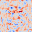
\includegraphics[width=\linewidth]{image0}
    \caption{Fran Drescher}
    \endminipage
    \hspace{10px}
    \minipage{0.32\textwidth}
    
\includegraphics[width=\linewidth]{image1}
    \caption{America Ferrera}
    \endminipage
    \hspace{10px}
    \minipage{0.32\textwidth}
    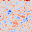
\includegraphics[width=\linewidth]{image2}
    \caption{Kristin Chenoweth}
    \endminipage
\end{figure}
\begin{figure}[h]   
    \minipage{0.32\textwidth}
    
\includegraphics[width=\linewidth]{image3}
    \caption{Alec Baldwin}
    \endminipage
    \hspace{10px}
    \minipage{0.32\textwidth}
    
\includegraphics[width=\linewidth]{image4}
    \caption{Bill Hader}
    \endminipage
    \hspace{10px}
    \minipage{0.32\textwidth}
    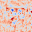
\includegraphics[width=\linewidth]{image5}
    \caption{Steve Carell}
    \endminipage
\end{figure}


\end{ProjectPart}
\clearpage

%----------------------------------------------------------------------------------------

\end{document}

